\chapter{Supporting Boogie Maps}
\label{sec:support-boogie-maps}

% Support Maps?
% - design the semantics
% - show properties
% - adjust proof generation
Extending the current proof generation to support Boogie maps requires several distinct steps.
First, we must design the formal semantics of Boogie maps to define their behavior.
This is a central component, as it dictates the ultimate proof obligations and establishes how the Boogie program is embedded within Isabelle.
After defining the semantics, we must prove that they satisfy our desired properties, particularly those generated by the verification conditions (VC).
Finally, we must adjust the proof generation module and related helper theorems to enable automatic proof generation for these new targets.


\section{Semantics: Stratification Datatype}

\subsection{Value Datatype}
\label{sec:where-to-start}

In the formal foundational Boogie semantics defined by the prior work in Isabelle/HOL
\footnote{https://github.com/viperproject/foundational-boogie},
there is a (polymorphic) value datatype, representing all values in the semantics.
This then used to define a state of the program,
with the current local and global state of the variables:

\begin{verbatim}
datatype lit =  LBool bool  | LInt int | LReal real

(* The values (and as a result the semantics)
are parametrized by the carrier type 'a for the abstract values
(values that have a type constructed via type constructors) *)

datatype 'a val = LitV lit | AbsV (the_absv: 'a)

type_synonym vname = nat (* variable name, de-bruijn index *)
type_synonym 'a named_state = "vname -> 'a val"

record 'a nstate =
  old_global_state :: "'a named_state"
  global_state :: "'a named_state"
  local_state :: "'a named_state"
  binder_state :: "nat -> 'a val"
\end{verbatim}

In Boogie maps are treated as first-class values.
Consequently, the initial step in supporting them involves extending the existing value datatype.
To incorporate Boogie Maps, we must introduce a new constructor to this datatype:

\begin{verbatim}
datatype 'a val = LitV lit | AbsV (the_absv: 'a) | MapV ?
\end{verbatim}

The question now is, how we should replace the \texttt{?}.

\subsection{Challenge: Cantor's Theorem}
\label{sec:cantor}

A naive approach to representing map values would involve a direct recursive definition:

\begin{verbatim}
datatype 'a val = LitV lit | AbsV (the_absv: 'a) | MapV "'a val => 'a val"
\end{verbatim}

However, Isabelle/HOL rejects this definition.
This is not a technical limitation of the tool, but a fundamental logical constraint.
Such a definition contradicts Cantor's Theorem,
which states that the cardinality of a function space $A \to A$ is strictly greater than the cardinality of $A$.
Since the constructor \texttt{MapV} would imply an injective function from the function space back into the value type,
it would lead to a logical inconsistency.

Notably, the issue arises specifically from the recursive occurrence of \texttt{'a val} in the domain (the left-hand side) of the function.
While a constructor like \texttt{bool => 'a val} is permissible, \texttt{'a val => bool} is not.

\subsection{Stratification Idea}
\label{sec:stratification-solution}
To resolve the conflict between recursion and cardinality, we propose an ``explicit unrolling'' of the recursion on the domain.
This creates a hierarchy of values:

\begin{itemize}
  \item Level 0: Contains only primitive values: literal and abstract values.
  \item Level 1: Maps with a domain of Level 0 and a range of Level 0 and Level 1.
  \item Level 2: Maps with a domain of Level 0 and Level 1 and a range of Level 0, 1, and 2.
  \item Level $n$: Maps where the domain is of level $\le n-1$ and the range is of level $\le n$.
\end{itemize}


This approach requires the user to explicitly specify the necessary nesting depth when defining the semantics.

To ensure the semantics can represent complex, nested Boogie map types,
it is essential that each level $n$ is cumulative, incorporating all preceding levels.
This allows the model to support maps where the keys or values are themselves maps of a lower level.
For instance, representing types such as
\lstinline[columns=fixed]{[int][[int]int]int} (a map of level 2, with a domain of level 0 and a range of level 2) or
\lstinline[columns=fixed]{[[[int]int]int]int} (a map of level 3, with a domain of level 2 and a range of level 0).

\begin{figure}[t]
  \centering
  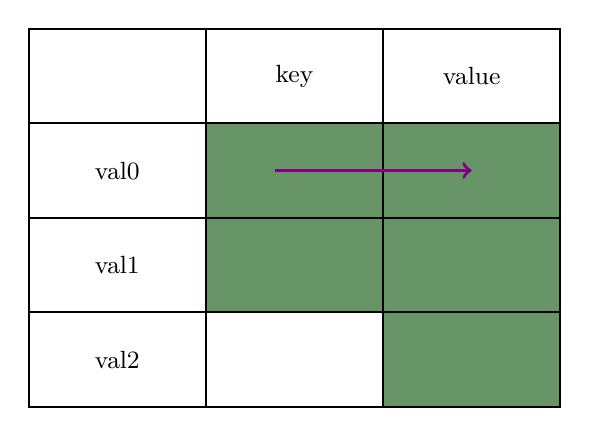
\begin{tikzpicture}[font=\small]
    \tikzstyle{gridbox}=[draw=black, thick, minimum width=2.25cm, minimum height=1.2cm, align=center]
    \tikzstyle{greenbox}=[gridbox, fill=green!30!black!60]

    \node[gridbox] at (0,0) {};
    \node[gridbox] at (2.25,0) {key};
    \node[gridbox] at (4.5,0) {value};

    \node[gridbox] at (0,-1.2) {val0};
    \node[greenbox] (k0) at (2.25,-1.2) {};
    \node[greenbox] (v0) at (4.5,-1.2) {};

    \node[gridbox] at (0,-2.4) {val1};
    \node[greenbox] at (2.25,-2.4) {};
    \node[greenbox] at (4.5,-2.4) {};

    \node[gridbox] at (0,-3.6) {val2};
    \node[gridbox] at (2.25,-3.6) {};
    \node[greenbox] at (4.5,-3.6) {};

    \draw[->, very thick, violet] (2,-1.2) -- (4.5,-1.2);
  \end{tikzpicture}
  \caption{Illustration of a stratified map of Level 2.
  It may take a value of level 0 or 1 as a key,
  and return values of level 0, 1 or 2.}
  \label{fig:stratified-map-hierarchy}
\end{figure}



\subsection{Stratification Datatype}
\label{sec:datatype-construction}
The stratified hierarchy could be implemented by defining discrete datatypes for each level:

\begin{verbatim}
datatype 'a val0 = LitV0 lit | AbsV0 (the_absv: 'a)
datatype 'a val1 = MapV1 "'a val0 => ('a val1 + 'a val0)"
datatype 'a val2 = MapV2 "('a val1 + 'a val0) => ('a val2 + 'a val1 + 'a val0)"
datatype 'a val3 = MapV3 "('a val2 + 'a val1 + 'a val0)
  => ('a val3 + 'a val2 + 'a val1 + 'a val0)"
\end{verbatim}

To minimize redundancy and improve maintainability, we introduce a helper datatype, \texttt{'k L},
which represents a functional map layer.
We then construct the hierarchy using type synonyms:

\begin{verbatim}
(* A helper datatype that takes a domain as a type parameter
   and provides a function from the domain to the domain and itself *)
datatype 'k L = FunL "'k => 'k L + 'k"

(* A datatype representing just primitive values *)
datatype 'a val0 = LitV0 lit | AbsV0 (the_absv: 'a)

(* Instantiate different map levels *)
type_synonym 'a val1 = "'a val0 L"
type_synonym 'a val2 = "('a val1 + 'a val0) L"
type_synonym 'a val3 = "('a val2 + 'a val1 + 'a val0) L"

type_synonym 'a val3210 = "'a val3 + 'a val2 + 'a val1 + 'a val0"
\end{verbatim}

To integrate these stratified levels into the core semantics,
we extend the primary \texttt{val} datatype with a generic \texttt{MapV} constructor.
By using a second type parameter, \texttt{'m}, we decouple the value definition from the specific map implementation:
\footnote{inspired by the initial attempt of the prior work
\url{https://github.com/viperproject/foundational-boogie/commit/c00254aa736513b3f243aa71182b44043e36c427}}


\begin{verbatim}
datatype ('a, 'm) val = LitV lit | AbsV (the_absv: 'a) | MapV 'm
\end{verbatim}

This allows us to instantiate the semantics with a specific number of levels:

\begin{verbatim}
(* Instantiate values with three map levels *)
type_synonym 'a val321  = "'a val3 + 'a val2 + 'a val1"
type_synonym 'a valn = "('a, 'a val321) val"
\end{verbatim}

Notably, \texttt{'a val0} is excluded from the \texttt{MapV} constructor,
as these represent primitive literals and abstract values, which are semantically distinct from map-based values.

However, establishing the datatype is only the foundational step;
we must subsequently define the functional operations and verify that they satisfy the required Boogie array axioms.
See Section~\ref{sec:vc-map-axioms}.

\subsection{Type of Values}
\label{sec:type-of-values}
A critical component of the value semantics, particularly for map operations such as \texttt{store} (Section~\ref{sec:store}) and well-formedness checks (Section~\ref{sec:wf-definition}),
is the \texttt{type\_of\_val} function.
This function determines the corresponding Boogie type for any given value within the semantics.
To support Boogie maps, the existing type definition must be extended to include a map type constructor:

\begin{verbatim}
datatype prim_ty
 = TBool | TInt | TReal

type_synonym tcon_id = string (* type constructor id *)

datatype ty
  = TVar nat | (* type variables as de-bruijn indices *)
    TPrim prim_ty | (* primitive types *)
    TCon tcon_id "ty list" (* type constructor *) |
    TMap ty ty (* maps *)
\end{verbatim}

As the current implementation is limited to single-arity maps
(Section~\ref{sec:goals-to-support}), the \texttt{TMap} constructor requires only two arguments:
the key type and the value type.
Supporting multi-arity maps would necessitate representing the keys as a list of types,
but the current dual-type representation is sufficient for our defined goals.

\paragraph{Type Ambiguity}
A challenge arises when implementing type extraction for map values.
Because our functional modeling of maps is extremely general,
a single internal Isabelle function could represent multiple distinct Boogie map types.
For instance, a map of type \texttt{val1} might contain a function mapping integers and booleans to integers and booleans,
making it impossible to distinguish from the outside whether it represents
a \texttt{[int]int}, \texttt{[bool]bool}, or \texttt{[int]bool} map.
To resolve this ambiguity, we explicitly store the intended key and value types within the map datatype:

\begin{isabellebody}
\isanewline
\isakeywordONE{datatype}\isamarkupfalse%
\ {\isacharprime}{\kern0pt}p\ L\ {\isacharequal}{\kern0pt}\ FunL\ {\isachardoublequoteopen}{\isacharprime}{\kern0pt}p\ {\isasymRightarrow}\ {\isacharprime}{\kern0pt}p\ L\ {\isacharplus}{\kern0pt}\ {\isacharprime}{\kern0pt}p{\isachardoublequoteclose}\ ty\ ty
\end{isabellebody}


While this ensures that every map value carries explicit type information,
it introduces a potential discrepancy:
there is no inherent semantic connection between the stored types and the actual behavior of the Isabelle function.
For example, a value could be tagged as \texttt{[bool]bool} while the underlying function operates on integers.
This consistency requirement is addressed later through the definition of well-formedness invariants (Section~\ref{sec:wf-definition}).

\paragraph{Accessor Functions for Map Types}
With the inclusion of explicit type tags,
we can define helper functions to extract the constituent types from a map type.
These functions are essential for the subsequent implementation of map operations:

\begin{verbatim}
fun key_ty where "key_ty (TMap tk _) = tk" | "key_ty _ = undefined"
fun val_ty where "val_ty (TMap _ tv) = tv" | "val_ty _ = undefined"
\end{verbatim}

Detailed definitions for the full \texttt{type\_of\_val} logic are provided in Appendix~\ref{sec:appendix}.

These functions also play a crucial role in satisfying the VC map axioms (Section~\ref{sec:vc-map-axioms}),
especially regarding $\MapType$, $\MapTypeInvK$, and $\MapTypeInvV$.



\section{Semantics: Well Formed Types}

The current datatype definition is too permissive
and does not inherently satisfy our required map axioms from Section~\ref{sec:vc-map-axioms}.
We must restrict them by enforcing additional well-formedness properties, denoted by \texttt{wf},
that the datatype must satisfy.


\subsection{Inductive Well-Formed Definition}
\label{sec:wf-definition}

The final inductive definition well-formed definition:

\begin{isabellebody}
\isanewline
\isakeywordONE{inductive}\isamarkupfalse%
\ wf\ \isakeywordTWO{where}\isanewline
\ \ \ \ wfLitV{\isacharcolon}{\kern0pt}\ {\isachardoublequoteopen}wf\ {\isacharparenleft}{\kern0pt}LitV\ v{\isacharparenright}{\kern0pt}{\isachardoublequoteclose}\ {\isacharbar}{\kern0pt}\ wfAbsV{\isacharcolon}{\kern0pt}\ {\isachardoublequoteopen}wf\ {\isacharparenleft}{\kern0pt}AbsV\ v{\isacharparenright}{\kern0pt}{\isachardoublequoteclose}\ {\isacharbar}{\kern0pt}\isanewline
\ \ \ \ wfMapV{\isacharcolon}{\kern0pt}\ {\isachardoublequoteopen}{\isasymlbrakk}\ wf{\isacharunderscore}{\kern0pt}ty\ m{\isacharsemicolon}{\kern0pt}\ \ {\isacharparenleft}{\kern0pt}{\isasymforall}k{\isachardot}{\kern0pt}\ wf\ {\isacharparenleft}{\kern0pt}selectImpl\ m\ k{\isacharparenright}{\kern0pt}{\isacharparenright}{\kern0pt}{\isacharsemicolon}{\kern0pt}\isanewline
\ \ \ \ \ \ {\isacharparenleft}{\kern0pt}{\isasymforall}k{\isachardot}{\kern0pt}\ {\isacharparenleft}{\kern0pt}{\isasymnot}wf\ k\ {\isasymor}\ type{\isacharunderscore}{\kern0pt}of{\isacharunderscore}{\kern0pt}val\ k\ {\isasymnoteq}\ key{\isacharunderscore}{\kern0pt}ty\ {\isacharparenleft}{\kern0pt}type{\isacharunderscore}{\kern0pt}of{\isacharunderscore}{\kern0pt}val\ m{\isacharparenright}{\kern0pt}{\isacharparenright}{\kern0pt}\isanewline 
\ \ \ \ \ \ \ \ \ \ \ {\isasymlongrightarrow}\ {\isacharparenleft}{\kern0pt}selectImpl\ m\ k{\isacharparenright}{\kern0pt}\ {\isacharequal}{\kern0pt}\ val{\isacharunderscore}{\kern0pt}of{\isacharunderscore}{\kern0pt}type\ {\isacharparenleft}{\kern0pt}val{\isacharunderscore}{\kern0pt}ty\ {\isacharparenleft}{\kern0pt}type{\isacharunderscore}{\kern0pt}of{\isacharunderscore}{\kern0pt}val\ m{\isacharparenright}{\kern0pt}{\isacharparenright}{\kern0pt}{\isacharparenright}{\kern0pt}{\isacharsemicolon}{\kern0pt}\isanewline
\ \ \ \ \ \ {\isacharparenleft}{\kern0pt}{\isasymforall}k{\isachardot}{\kern0pt}\ type{\isacharunderscore}{\kern0pt}of{\isacharunderscore}{\kern0pt}val\ {\isacharparenleft}{\kern0pt}selectImpl\ m\ k{\isacharparenright}{\kern0pt}\ {\isacharequal}{\kern0pt}\ val{\isacharunderscore}{\kern0pt}ty\ {\isacharparenleft}{\kern0pt}type{\isacharunderscore}{\kern0pt}of{\isacharunderscore}{\kern0pt}val\ m{\isacharparenright}{\kern0pt}{\isacharparenright}{\kern0pt}\isanewline
\ \ \ \ \ \ {\isasymrbrakk}\ {\isasymLongrightarrow}\ wf\ m{\isachardoublequoteclose}
\end{isabellebody}

First, we define primitive types, such as literal and abstract values,
as well-formed.
Those are our base cases for our inductive definition.
For a map to be well-formed it has to satisfy four properties.


\subsection{Closedness of Select \& Store}
\label{sec:closed}

If we use a constrained type and apply operations like select or store,
the result should be constrained as well; i.e., it must satisfy our desired properties.
Thus, one fundamental requirement is \isa{(\isasymforall k. wf k --> wf (selectImpl m k))}.
\footnote{Assuming we have a suitable definition of \texttt{selectImpl}, which will be introduced in Section~\ref{sec:select}.}

We observe that the definition of \texttt{wf} is dependent on the \texttt{wf} of other values.
For a recursive definition, we would need to guarantee termination
(e.g., applying \texttt{wf} only to strictly 'smaller' terms).
This is non-trivial here because \texttt{selectImpl m k} may return an arbitrary value.
Fortunately, Isabelle/HOL provides \texttt{inductive} definitions,
\ref{sec:isabelle}
allowing us to characterize \texttt{wf} values based on previously determined \texttt{wf} values.

A recursive \texttt{wf} call is not permitted in a negative position. This presents a challenge since:
\texttt{(ALL k. wf k --> wf (selectImpl m k))} logically translates to \texttt{(ALL k. ¬ wf k OR wf (selectImpl m k))}.
This restriction also makes intuitive sense, as our inductive definition can construct proofs that values are \texttt{wf},
but not that they are \texttt{¬wf}.
Our solution is to strengthen the property by dropping the antecedent,
enforcing that the result is always \texttt{wf}, regardless of whether the key is \texttt{wf} or not.

\begin{verbatim}
  (ALL k. wf (selectImpl m k))
\end{verbatim}

For the store operation, we do not require an additional structural property within the inductive definition, as we can independently derive the lemma:
\texttt{(ALL k v. wf m AND wf k AND wf v --> wf (storeImpl m k v))}.


\subsection{Type Safety}
\label{sec:type-safety}
From the VC map axiom (\ref{ax:map-select-typesafe}),
we require the property that if we select from a map using a key of the map's designated domain type,
the result is of the map's range type.
In Isabelle, this translates to:

\begin{verbatim}
(ALL k. wf k AND type_of_val k = key_ty (type_of_val m)
--> type_of_val (selectImpl m k) = val_ty (type_of_val m))
\end{verbatim}

%[mention why it is hard to do that structurally using datatypes only?]

We will actually enforce a stronger condition explicitly:

\begin{verbatim}
(ALL k. type_of_val (selectImpl m k) = val_ty (type_of_val m))
\end{verbatim}

One reason for this, again, is that \texttt{wf} may not appear in a negative position
(in this case, on the left-hand side of an implication).
The weaker version will be a derived property, deduced by combining the stronger condition with our other constraints.
Enforcing this explicitly is more convenient, as it provides a stronger guarantee when building nested maps and proving their well-formedness.


\subsection{No Duplicate Representation}
\label{sec:no-duplicate}

As discussed in Section~\ref{sec:goals-to-support}, we require our maps to be extensional.
More concretely, this means there must be a unique Isabelle representation for each Boogie map.
If two map values agree on all keys, they should be represented by the identical Isabelle term.
The naive definition presents two primary issues in satisfying this property.

\paragraph{Problem 1: Low-level map as a high-level value}
Consider an \texttt{[int]int} map in Boogie.
We want to canonically represent this in Isabelle as a value of level 1 (i.e., \texttt{'a val1}).
Unfortunately, there is nothing to prevent us from representing it as a map at level 3 (i.e., \texttt{'a val3}), since level 3 structurally subsumes \texttt{'a val0} in both its domain and range.
Consequently, we possess multiple ways to represent the exact same semantic map.

\paragraph{Solution: Type Hierarchies}
To prevent this ambiguity, we enforce a strict type hierarchy: map types at level $n$ must have either their domain at level $n-1$ or their range at level $n$.

% tmap_lvl, wf_L, wf_ty
\begin{isabellebody}
\isanewline
\isakeywordONE{fun}\isamarkupfalse%
\ tmap{\isacharunderscore}{\kern0pt}lvl\ {\isacharcolon}{\kern0pt}{\isacharcolon}{\kern0pt}\ {\isachardoublequoteopen}ty\ {\isasymRightarrow}\ nat{\isachardoublequoteclose}\ \isakeywordTWO{where}\isanewline
\ \ \ \ {\isachardoublequoteopen}tmap{\isacharunderscore}{\kern0pt}lvl\ {\isacharparenleft}{\kern0pt}TMap\ tk\ tv{\isacharparenright}{\kern0pt}\ {\isacharequal}{\kern0pt}\ max\ {\isacharparenleft}{\kern0pt}{\isadigit{1}}\ {\isacharplus}{\kern0pt}\ tmap{\isacharunderscore}{\kern0pt}lvl\ tk{\isacharparenright}{\kern0pt}\ {\isacharparenleft}{\kern0pt}tmap{\isacharunderscore}{\kern0pt}lvl\ tv{\isacharparenright}{\kern0pt}{\isachardoublequoteclose}\isanewline
\ \ {\isacharbar}{\kern0pt}\ {\isachardoublequoteopen}tmap{\isacharunderscore}{\kern0pt}lvl\ {\isacharunderscore}{\kern0pt}\ {\isacharequal}{\kern0pt}\ {\isadigit{0}}{\isachardoublequoteclose}\isanewline
\isanewline
\isakeywordONE{primrec}\isamarkupfalse%
\ wf{\isacharunderscore}{\kern0pt}L\ \isakeywordTWO{where}\isanewline
\ \ {\isachardoublequoteopen}wf{\isacharunderscore}{\kern0pt}L\ n\ {\isacharparenleft}{\kern0pt}FunL\ {\isacharunderscore}{\kern0pt}\ tk\ tv{\isacharparenright}{\kern0pt}\ {\isacharequal}{\kern0pt}\ {\isacharparenleft}{\kern0pt}\isanewline
\ \ \ \ {\isacharparenleft}{\kern0pt}tmap{\isacharunderscore}{\kern0pt}lvl\ tk\ {\isasymle}\ n{\isacharminus}{\kern0pt}{\isadigit{1}}{\isacharparenright}{\kern0pt}\ {\isasymand}\ {\isacharparenleft}{\kern0pt}tmap{\isacharunderscore}{\kern0pt}lvl\ tv\ {\isasymle}\ n{\isacharparenright}{\kern0pt}\ {\isasymand}\isanewline
\ \ \ \ {\isacharparenleft}{\kern0pt}{\isacharparenleft}{\kern0pt}tmap{\isacharunderscore}{\kern0pt}lvl\ tk\ {\isacharequal}{\kern0pt}\ n{\isacharminus}{\kern0pt}{\isadigit{1}}{\isacharparenright}{\kern0pt}\ {\isasymor}\ {\isacharparenleft}{\kern0pt}tmap{\isacharunderscore}{\kern0pt}lvl\ tv\ {\isacharequal}{\kern0pt}\ n{\isacharparenright}{\kern0pt}{\isacharparenright}{\kern0pt}{\isacharparenright}{\kern0pt}{\isachardoublequoteclose}\ \ \isanewline
\isanewline
\isakeywordONE{fun}\isamarkupfalse%
\ wf{\isacharunderscore}{\kern0pt}ty\ {\isacharcolon}{\kern0pt}{\isacharcolon}{\kern0pt}\ {\isachardoublequoteopen}{\isacharprime}{\kern0pt}a\ valn\ {\isasymRightarrow}\ bool{\isachardoublequoteclose}\ \isakeywordTWO{where}\isanewline
\ \ \ \ {\isachardoublequoteopen}wf{\isacharunderscore}{\kern0pt}ty\ {\isacharparenleft}{\kern0pt}LitV\ v{\isacharparenright}{\kern0pt}\ {\isacharequal}{\kern0pt}\ True{\isachardoublequoteclose}\isanewline
\ \ {\isacharbar}{\kern0pt}\ {\isachardoublequoteopen}wf{\isacharunderscore}{\kern0pt}ty\ {\isacharparenleft}{\kern0pt}AbsV\ v{\isacharparenright}{\kern0pt}\ {\isacharequal}{\kern0pt}\ True{\isachardoublequoteclose}\isanewline
\ \ {\isacharbar}{\kern0pt}\ {\isachardoublequoteopen}wf{\isacharunderscore}{\kern0pt}ty\ {\isacharparenleft}{\kern0pt}MapV\ {\isacharparenleft}{\kern0pt}Inr\ {\isacharparenleft}{\kern0pt}Inr\ m{\isacharparenright}{\kern0pt}{\isacharparenright}{\kern0pt}{\isacharparenright}{\kern0pt}\ {\isacharequal}{\kern0pt}\ wf{\isacharunderscore}{\kern0pt}L\ {\isadigit{1}}\ m{\isachardoublequoteclose}\isanewline
\ \ {\isacharbar}{\kern0pt}\ {\isachardoublequoteopen}wf{\isacharunderscore}{\kern0pt}ty\ {\isacharparenleft}{\kern0pt}MapV\ {\isacharparenleft}{\kern0pt}Inr\ {\isacharparenleft}{\kern0pt}Inl\ m{\isacharparenright}{\kern0pt}{\isacharparenright}{\kern0pt}{\isacharparenright}{\kern0pt}\ {\isacharequal}{\kern0pt}\ wf{\isacharunderscore}{\kern0pt}L\ {\isadigit{2}}\ m{\isachardoublequoteclose}\isanewline
\ \ {\isacharbar}{\kern0pt}\ {\isachardoublequoteopen}wf{\isacharunderscore}{\kern0pt}ty\ {\isacharparenleft}{\kern0pt}MapV\ {\isacharparenleft}{\kern0pt}Inl\ m{\isacharparenright}{\kern0pt}{\isacharparenright}{\kern0pt}\ {\isacharequal}{\kern0pt}\ wf{\isacharunderscore}{\kern0pt}L\ {\isadigit{3}}\ m{\isachardoublequoteclose}
\end{isabellebody}

\begin{figure}[t]
  \centering
  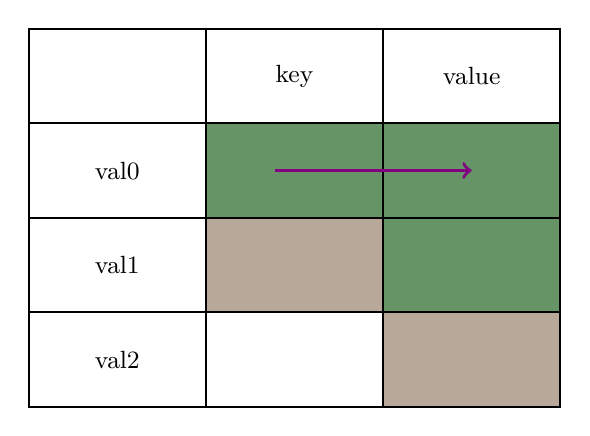
\begin{tikzpicture}[font=\small]
    \tikzstyle{gridbox}=[draw=black, thick, minimum width=2.25cm, minimum height=1.2cm, align=center]
    \tikzstyle{greenbox}=[gridbox, fill=green!30!black!60]
    \tikzstyle{orangebox}=[gridbox, fill=orange!30!black!40]

    \node[gridbox] at (0,0) {};
    \node[gridbox] at (2.25,0) {key};
    \node[gridbox] at (4.5,0) {value};

    \node[gridbox] at (0,-1.2) {val0};
    \node[greenbox] (k0) at (2.25,-1.2) {};
    \node[greenbox] (v0) at (4.5,-1.2) {};

    \node[gridbox] at (0,-2.4) {val1};
    \node[orangebox] at (2.25,-2.4) {};
    \node[greenbox] at (4.5,-2.4) {};

    \node[gridbox] at (0,-3.6) {val2};
    \node[gridbox] at (2.25,-3.6) {};
    \node[orangebox] at (4.5,-3.6) {};

    \draw[->, very thick, violet] (2,-1.2) -- (4.5,-1.2);
  \end{tikzpicture}
  \caption{Illustration of a stratified map of Level 2.
  Its domain type either has to be of level 1
  or its range type of level 2.}
  \label{fig:stratified-map-hierarchy}
\end{figure}

\paragraph{Problem 2: Function behavior outside the domain}
Consider the Boogie map \texttt{(lambda x: int :: x+1)}.
In its Isabelle embedding, the domain is not rigidly constrained to integers only.
Therefore, we might construct two maps that execute identically on integers but differ when applied to booleans.
To guarantee extensionality, we must ensure that maps sharing the same Boogie behavior also execute identically outside their intended domain. 

A robust solution is to enforce a sentinel value for all keys residing outside the expected domain.
It is important to note that "values outside the intended domain" include not only values of the wrong type but also values that are not well-formed.
Consequently, we enforce a property of the following form:

\begin{isabellebody}
{\isasymforall}k{\isachardot}{\kern0pt}\ {\isacharparenleft}{\kern0pt}{\isasymnot}wf\ k\ {\isasymor}\ type{\isacharunderscore}{\kern0pt}of{\isacharunderscore}{\kern0pt}val\ k\ {\isasymnoteq}\ key{\isacharunderscore}{\kern0pt}ty\ {\isacharparenleft}{\kern0pt}type{\isacharunderscore}{\kern0pt}of{\isacharunderscore}{\kern0pt}val\ m{\isacharparenright}{\kern0pt}{\isacharparenright}{\kern0pt}\ {\isasymlongrightarrow}\ {\isacharparenleft}{\kern0pt}selectImpl\ m\ k{\isacharparenright}{\kern0pt}\ {\isacharequal}{\kern0pt}\ sentinel?{\kern0pt}
\end{isabellebody}

The question remains: what should this \texttt{sentinel?} value be? As established in Section~\ref{sec:type-safety}, we cannot cleanly perform a case distinction on \texttt{wf k} because \texttt{wf} is not permitted in a negative position.
Thus, if presented with a key \texttt{k} of unknown well-formedness, we cannot statically determine whether \texttt{type\_of\_val (selectImpl m k) = val\_ty (type\_of\_val m)} should hold, or if \texttt{type\_of\_val (selectImpl m k) = sentinel?} applies. 

However, if the \texttt{sentinel?} itself is of type \texttt{val\_ty (type\_of\_val m)}, both conditions unify seamlessly.
We leverage the helper function \texttt{val\_of\_type}, which returns a default value of a given type, to generate our sentinel:\\
\texttt{sentinel? = val\_of\_type (val\_ty (type\_of\_val m))}

\begin{table}[t]
\begin{tabular}{|l|l|l|}
  \hline
                 & \texttt{k} has correct type & \texttt{k} has incorrect type \\ \hline
  \texttt{wf k}  & \texttt{(selectImpl m k)} has correct type & \texttt{sentinel}  \\ \hdashline
\texttt{\textasciitilde wf k}  & \texttt{sentinel}    & \texttt{sentinel}  \\ \hline
\end{tabular}

  \caption{Cases in which we must return a sentinel value and cases in which the return type must be correct.
  The dashed line represents our inability to distinguish by cases on \texttt{wf k}.}
  \label{tab:sentinel-cases}
\end{table}

\subsection{Well-Formed Type Definition}
\label{sec:constrained-types}

Using our well-formed definition\ref{sec:wf-definition},
we can create a new 'constrained' type
via the \texttt{typedef} command in Isabelle.\ref{sec:isabelle}

\begin{verbatim}
definition wf_map_set :: "'a val321 set" where
"wf_map_set = {m. wf (MapV m)}"

typedef (overloaded) 'a wf_maps = "wf_map_set :: 'a val321 set"
<proof>
  (* showing some witness, such that wf_maps is not empty *)

type_synonym 'a wf_val = "('a, 'a wf_maps) val"
\end{verbatim}

Showing a witness for maps requires some non-trivial work,
which we leave out for brevity.


\section{Semantics: Map Operations}
\subsection{Internal Datatype Conversion}
\label{sec:conversion-internal}
% [TODO should this just be in the appendix?]

The stratified levels introduced for our map semantics (Section~\ref{sec:stratification-solution}) are an implementation detail that should be abstracted away from the broader semantics.
For this reason, we structured the primary \texttt{val} datatype generically (Section~\ref{sec:datatype-construction}).

To operationalize this, we require translator functions to convert between the generic \texttt{val} representation and our explicit level-based sum types:

% [TODO potentially simplify sum semantics, i.e. Inr (Inl x) -> In2 x]
\begin{verbatim}
fun toVal3210 :: "'a valn => 'a val3210" where
    "toVal3210 (LitV v) = (Inr (Inr (Inr (LitV0 v))))"
  | "toVal3210 (AbsV v) = (Inr (Inr (Inr (AbsV0 v))))"
  | "toVal3210 (MapV (Inr (Inr m))) = (Inr (Inr (Inl m)))"
  | "toVal3210 (MapV (Inr (Inl m))) = (Inr (Inl m))"
  | "toVal3210 (MapV (Inl m)) = (Inl m)"

fun val3ToValn :: "'a val3210 => 'a valn" where
    "val3ToValn (Inr (Inr (Inr (LitV0 v)))) = (LitV v)"
  | "val3ToValn (Inr (Inr (Inr (AbsV0 v)))) = (AbsV v)"
  | "val3ToValn (Inr (Inr (Inl m))) = (MapV (Inr (Inr m)))"
  | "val3ToValn (Inr (Inl m)) = (MapV (Inr (Inl m)))"
  | "val3ToValn (Inl m) = (MapV (Inl m))"
\end{verbatim}

\subsection{Select Semantics}
\label{sec:select}

We now formally define the select function for our map semantics. We begin with an auxiliary function that executes the core logic over the internal level representations:

% [TODO potentially simplify semantics: remove primitive cases, move default case to non-aux function to avoid conversions]
\begin{verbatim}
fun selectImplAux :: "'a val3210 => 'a val3210 => 'a val3210" where
    "selectImplAux (Inr (Inr (Inr (LitV0 v)))) _ = (Inr (Inr (Inr undefined)))"
  | "selectImplAux (Inr (Inr (Inr (AbsV0 v)))) _ = (Inr (Inr (Inr undefined)))"
  | "selectImplAux (Inr (Inr (Inl (FunL m _ _)))) (Inr (Inr (Inr k))) = Inr (Inr (m k))"
  | "selectImplAux (Inr (Inl (FunL m _ _))) (Inr (Inr k)) = Inr (m k)"
  | "selectImplAux (Inl (FunL m _ _)) (Inr k) = (m k)"
  | "selectImplAux m _ = toVal3210 (val_of_type (val_ty (type_of_val (val3ToValn m))))"
\end{verbatim}

% \texttt{absval} is a type class, that is needed to call \texttt{type\_of\_val}.
% This is addressed later in Section~\ref{sec:proofgen-module}.

Consider the case \texttt{"selectImplAux (Inr (Inl (FunL m \_ \_))) (Inr (Inr k)) = Inr (m k)"}.
This represents evaluating a map residing at level $2$ with a key of level $\le 1$.
Here, \texttt{m} is a function mapping values of level $\le 1$ to values of level $\le 2$.
Consequently, the application \texttt{m k} yields a value of level $\le 2$, and the \texttt{Inr} constructor ensures the final result conforms to the overall type \texttt{'a val3210}.
The logic for the remaining map levels is analogous.

For primitive value cases, the specific return value is inconsequential, (provided it is well-formed, ensuring that \texttt{selectImpl} remains closed under \texttt{wf}, see Section~\ref{sec:wf-definition}).
We opt to return an \texttt{undefined}\footnote{More accurately described as unspecified rather than literally undefined.} primitive value, as all such values trivially satisfy well-formedness.

If an evaluation encounters a key from an unsupported level, the function gracefully falls back to returning the map's sentinel value, thereby preserving all required well-formedness invariants.

With this robust auxiliary function established, the primary select function simply wraps the required type conversions:

\begin{isabellebody}
\isanewline
\isakeywordONE{fun}\isamarkupfalse%
\ selectImpl\ {\isacharcolon}{\kern0pt}{\isacharcolon}{\kern0pt}\ {\isachardoublequoteopen}{\isacharprime}{\kern0pt}a{\isacharcolon}{\kern0pt}{\isacharcolon}{\kern0pt}absval\ valn\ {\isasymRightarrow}\ {\isacharprime}{\kern0pt}a\ valn\ {\isasymRightarrow}\ {\isacharprime}{\kern0pt}a\ valn{\isachardoublequoteclose}\ \isakeywordTWO{where}\isanewline
\ \ {\isachardoublequoteopen}selectImpl\ m\ k\ {\isacharequal}{\kern0pt}\ val{\isadigit{3}}ToValn\ {\isacharparenleft}{\kern0pt}selectImplAux\ {\isacharparenleft}{\kern0pt}toVal{\isadigit{3}}{\isadigit{2}}{\isadigit{1}}{\isadigit{0}}\ m{\isacharparenright}{\kern0pt}\ {\isacharparenleft}{\kern0pt}toVal{\isadigit{3}}{\isadigit{2}}{\isadigit{1}}{\isadigit{0}}\ k{\isacharparenright}{\kern0pt}{\isacharparenright}{\kern0pt}{\isachardoublequoteclose}\end{isabellebody}


\subsection{Store Semantics}
\label{sec:store}

The store operation follows a similar methodology, beginning with an auxiliary functional update over the internal representation:

\begin{isabellebody}
\isanewline
\isakeywordONE{fun}\isamarkupfalse%
\ storeImplAux\ {\isacharcolon}{\kern0pt}{\isacharcolon}{\kern0pt}\ {\isachardoublequoteopen}{\isacharprime}{\kern0pt}a\ val{\isadigit{3}}{\isadigit{2}}{\isadigit{1}}{\isadigit{0}}\ {\isasymRightarrow}\ {\isacharprime}{\kern0pt}a\ val{\isadigit{3}}{\isadigit{2}}{\isadigit{1}}{\isadigit{0}}\ {\isasymRightarrow}\ {\isacharprime}{\kern0pt}a\ val{\isadigit{3}}{\isadigit{2}}{\isadigit{1}}{\isadigit{0}}\ {\isasymRightarrow}\ {\isacharprime}{\kern0pt}a\ val{\isadigit{3}}{\isadigit{2}}{\isadigit{1}}{\isadigit{0}}{\isachardoublequoteclose}\ \isakeywordTWO{where}\isanewline
\ \ \ \ {\isachardoublequoteopen}storeImplAux\ {\isacharparenleft}{\kern0pt}Inr\ {\isacharparenleft}{\kern0pt}Inr\ {\isacharparenleft}{\kern0pt}Inl\ {\isacharparenleft}{\kern0pt}FunL\ m\ tk\ tv{\isacharparenright}{\kern0pt}{\isacharparenright}{\kern0pt}{\isacharparenright}{\kern0pt}{\isacharparenright}{\kern0pt}\ {\isacharparenleft}{\kern0pt}Inr\ {\isacharparenleft}{\kern0pt}Inr\ {\isacharparenleft}{\kern0pt}Inr\ k{\isacharparenright}{\kern0pt}{\isacharparenright}{\kern0pt}{\isacharparenright}{\kern0pt}\ {\isacharparenleft}{\kern0pt}Inr\ {\isacharparenleft}{\kern0pt}Inr\ v{\isacharparenright}{\kern0pt}{\isacharparenright}{\kern0pt}\isanewline
\ \ \ \ \ \ {\isacharequal}{\kern0pt}\ {\isacharparenleft}{\kern0pt}Inr\ {\isacharparenleft}{\kern0pt}Inr\ {\isacharparenleft}{\kern0pt}Inl\ {\isacharparenleft}{\kern0pt}FunL\ {\isacharparenleft}{\kern0pt}m{\isacharparenleft}{\kern0pt}k\ {\isacharcolon}{\kern0pt}{\isacharequal}{\kern0pt}\ v{\isacharparenright}{\kern0pt}{\isacharparenright}{\kern0pt}\ tk\ tv{\isacharparenright}{\kern0pt}{\isacharparenright}{\kern0pt}{\isacharparenright}{\kern0pt}{\isacharparenright}{\kern0pt}{\isachardoublequoteclose}\isanewline
\ \ {\isacharbar}{\kern0pt}\ {\isachardoublequoteopen}storeImplAux\ {\isacharparenleft}{\kern0pt}Inr\ {\isacharparenleft}{\kern0pt}Inl\ {\isacharparenleft}{\kern0pt}FunL\ m\ tk\ tv{\isacharparenright}{\kern0pt}{\isacharparenright}{\kern0pt}{\isacharparenright}{\kern0pt}\ {\isacharparenleft}{\kern0pt}Inr\ {\isacharparenleft}{\kern0pt}Inr\ k{\isacharparenright}{\kern0pt}{\isacharparenright}{\kern0pt}\ {\isacharparenleft}{\kern0pt}Inr\ v{\isacharparenright}{\kern0pt}\isanewline
\ \ \ \ \ \ {\isacharequal}{\kern0pt}\ {\isacharparenleft}{\kern0pt}Inr\ {\isacharparenleft}{\kern0pt}Inl\ {\isacharparenleft}{\kern0pt}FunL\ {\isacharparenleft}{\kern0pt}m{\isacharparenleft}{\kern0pt}k\ {\isacharcolon}{\kern0pt}{\isacharequal}{\kern0pt}\ v{\isacharparenright}{\kern0pt}{\isacharparenright}{\kern0pt}\ tk\ tv{\isacharparenright}{\kern0pt}{\isacharparenright}{\kern0pt}{\isacharparenright}{\kern0pt}{\isachardoublequoteclose}\isanewline
\ \ {\isacharbar}{\kern0pt}\ {\isachardoublequoteopen}storeImplAux\ {\isacharparenleft}{\kern0pt}Inl\ {\isacharparenleft}{\kern0pt}FunL\ m\ tk\ tv{\isacharparenright}{\kern0pt}{\isacharparenright}{\kern0pt}\ {\isacharparenleft}{\kern0pt}Inr\ k{\isacharparenright}{\kern0pt}\ v\isanewline
\ \ \ \ \ \ {\isacharequal}{\kern0pt}\ {\isacharparenleft}{\kern0pt}Inl\ {\isacharparenleft}{\kern0pt}FunL\ {\isacharparenleft}{\kern0pt}m{\isacharparenleft}{\kern0pt}k\ {\isacharcolon}{\kern0pt}{\isacharequal}{\kern0pt}\ v{\isacharparenright}{\kern0pt}{\isacharparenright}{\kern0pt}\ tk\ tv{\isacharparenright}{\kern0pt}{\isacharparenright}{\kern0pt}{\isachardoublequoteclose}\isanewline
\ \ {\isacharbar}{\kern0pt}\ {\isachardoublequoteopen}storeImplAux\ x\ {\isacharunderscore}{\kern0pt}\ {\isacharunderscore}{\kern0pt}\ {\isacharequal}{\kern0pt}\ x{\isachardoublequoteclose}
\end{isabellebody}

As before, we pattern-match across each map level and its corresponding supported key levels.
However, rather than function application, we execute a function update (\texttt{k := v}).
If the key level is absent from the domain, or if the update targets a primitive value, the function safely returns the unmodified value.

The actual \texttt{storeImpl} function performs a critical additional check beyond basic type conversion:

\begin{isabellebody}
\isanewline
\isakeywordONE{fun}\isamarkupfalse%
\ storeImpl\ {\isacharcolon}{\kern0pt}{\isacharcolon}{\kern0pt}\ {\isachardoublequoteopen}{\isacharprime}{\kern0pt}a{\isacharcolon}{\kern0pt}{\isacharcolon}{\kern0pt}absval\ valn\ {\isasymRightarrow}\ {\isacharprime}{\kern0pt}a\ valn\ {\isasymRightarrow}\ {\isacharprime}{\kern0pt}a\ valn\ {\isasymRightarrow}\ {\isacharprime}{\kern0pt}a\ valn{\isachardoublequoteclose}\ \isakeywordTWO{where}\isanewline
\ \ {\isachardoublequoteopen}storeImpl\ m\ k\ v\ {\isacharequal}{\kern0pt}\ {\isacharparenleft}{\kern0pt}if\ type{\isacharunderscore}{\kern0pt}of{\isacharunderscore}{\kern0pt}val\ m\ {\isacharequal}{\kern0pt}\ TMap\ {\isacharparenleft}{\kern0pt}type{\isacharunderscore}{\kern0pt}of{\isacharunderscore}{\kern0pt}val\ k{\isacharparenright}{\kern0pt}\ {\isacharparenleft}{\kern0pt}type{\isacharunderscore}{\kern0pt}of{\isacharunderscore}{\kern0pt}val\ v{\isacharparenright}{\kern0pt}\isanewline
\ \ \ \ then\ val{\isadigit{3}}ToValn\ {\isacharparenleft}{\kern0pt}storeImplAux\ {\isacharparenleft}{\kern0pt}toVal{\isadigit{3}}{\isadigit{2}}{\isadigit{1}}{\isadigit{0}}\ m{\isacharparenright}{\kern0pt}\ {\isacharparenleft}{\kern0pt}toVal{\isadigit{3}}{\isadigit{2}}{\isadigit{1}}{\isadigit{0}}\ k{\isacharparenright}{\kern0pt}\ {\isacharparenleft}{\kern0pt}toVal{\isadigit{3}}{\isadigit{2}}{\isadigit{1}}{\isadigit{0}}\ v{\isacharparenright}{\kern0pt}{\isacharparenright}{\kern0pt}\isanewline
\ \ \ \ else\ m{\isacharparenright}{\kern0pt}{\isachardoublequoteclose}
\end{isabellebody}

It ensures the update is exclusively executed when the types explicitly match.
Omitting this check would risk a violation of the established well-formedness properties.


\section{Proof of Properties}

\subsection{Our VC antecedent change} \mbox{}\\
\label{sec:our-vc-change}

The current axiom governing map updates \eqref{ax:map-update-strong}
is too strong for our semantics,
which relies on our stratification solution (Section~\ref{sec:stratification-solution}).
The primary issue is that this axiom must hold for every value $m$,
even if it is not a map, and for every value $k$,
even if its type does not match the domain type of $m$.
Accordingly, we weaken the axiom:

\begin{equation}
  \label{ax:map-update-weak}
  \begin{aligned}
    &\forall \ m \ k \ v.\\
    &\type\ v = \MapTypeInvV\ (\type\ m)\\
    &\type\ m = \MapType\ (\type\ k)\ (\type\ v)\\
    &\implies  \Select\ (\Store\ m\ k\ v)\ k = v
  \end{aligned}
\end{equation}

With $\type\ m = \MapType\ (\type\ k)\ (\type\ v)$, we guarantee
that $m$ is indeed a map and that the store operation is applied to values of the appropriate types.
This changes the VC produced by the Boogie verifier
and may therefore reduce the number of successful verifications.
We expect it to work in many cases, since the input programs are type-checked.
Nonetheless, the solver has a weaker axiom available,
so we must evaluate whether it is in fact too weak.
% TODO evaluation


\subsection{Showing Desired Properties}
\label{sec:typedef-lifting}

Having formalized the datatype, well-formedness, select, and store operations, we must now demonstrate that they satisfy our theoretical goals, specifically the VC map axioms detailed in Section~\ref{sec:vc-map-axioms}.
As discussed in Section~\ref{sec:constrained-types}, we embed our well-formedness properties directly into a new constrained type.
We must then "lift" our select and store functions, alongside their proven lemmas, so that they operate seamlessly on this new type.
We have successfully proven the following lemmas.

We first show, that our map operations are closed under well-formedness:

\begin{isabellebody}
\isakeywordONE{lemma}\isamarkupfalse%
\ selectClosedWf{\isacharcolon}{\kern0pt}
{\isachardoublequoteopen}wf\ m {\isasymRightarrow}\ wf\ {\isacharparenleft}{\kern0pt}selectImpl\ m\ k{\isacharparenright}{\kern0pt}{\isachardoublequoteclose}\isanewline

\isakeywordONE{lemma}\isamarkupfalse%
\ storeClosedWf{\isacharcolon}{\kern0pt}
{\isachardoublequoteopen}[wf\ m, wf\ k,\ wf\ v] {\isasymRightarrow}\ wf\ {\isacharparenleft}{\kern0pt}storeImpl\ m\ k{\isacharparenright}{\kern0pt}{\isachardoublequoteclose}\isanewline
\end{isabellebody}

With the help of these lemmas we are able to \emph{lift} our operations to our new type:
\begin{isabellebody}
\isakeywordONE{lift{\isacharunderscore}{\kern0pt}definition}\isamarkupfalse%
\ wf{\isacharunderscore}{\kern0pt}select\ {\isacharcolon}{\kern0pt}{\isacharcolon}{\kern0pt}\ {\isachardoublequoteopen}{\isacharprime}{\kern0pt}a{\isacharcolon}{\kern0pt}{\isacharcolon}{\kern0pt}absval\ wf{\isacharunderscore}{\kern0pt}val\ {\isasymRightarrow}\ {\isacharprime}{\kern0pt}a\ wf{\isacharunderscore}{\kern0pt}val\ {\isasymRightarrow}\ {\isacharprime}{\kern0pt}a\ wf{\isacharunderscore}{\kern0pt}val{\isachardoublequoteclose}\isanewline
\ \ \isakeywordTWO{is}\ selectImpl\isanewline
<proof>\isanewline

\isakeywordONE{lift{\isacharunderscore}{\kern0pt}definition}\isamarkupfalse%
\ wf{\isacharunderscore}{\kern0pt}store\ {\isacharcolon}{\kern0pt}{\isacharcolon}{\kern0pt}\ {\isachardoublequoteopen}{\isacharprime}{\kern0pt}a{\isacharcolon}{\kern0pt}{\isacharcolon}{\kern0pt}absval\ wf{\isacharunderscore}{\kern0pt}val\ {\isasymRightarrow}\ {\isacharprime}{\kern0pt}a\ wf{\isacharunderscore}{\kern0pt}val\ {\isasymRightarrow}\ {\isacharprime}{\kern0pt}a\ wf{\isacharunderscore}{\kern0pt}val\ {\isasymRightarrow}\ {\isacharprime}{\kern0pt}a\ wf{\isacharunderscore}{\kern0pt}val{\isachardoublequoteclose}\isanewline
\ \ \isakeywordTWO{is}\ storeImpl\isanewline
<proof>\isanewline
\end{isabellebody}


Then we want to show that our type satisfies the VC axioms\ref{sec:vc-map-axioms}.

\begin{isabellebody}
\isakeywordONE{lemma}\isamarkupfalse%
\ ArrayAxUpdate{\isacharcolon}{\kern0pt}\isanewline
\ \ \isakeywordTWO{assumes}\ {\isachardoublequoteopen}wf\ M{\isachardoublequoteclose}\isanewline
\ \ \isakeywordTWO{assumes}\ {\isachardoublequoteopen}wf\ k{\isachardoublequoteclose}\isanewline
\ \ \isakeywordTWO{assumes}\ {\isachardoublequoteopen}wf\ v{\isachardoublequoteclose}\isanewline
\ \ \isakeywordTWO{assumes}\ {\isachardoublequoteopen}type{\isacharunderscore}{\kern0pt}of{\isacharunderscore}{\kern0pt}val\ M\ {\isacharequal}{\kern0pt}\ TMap\ {\isacharparenleft}{\kern0pt}type{\isacharunderscore}{\kern0pt}of{\isacharunderscore}{\kern0pt}val\ k{\isacharparenright}{\kern0pt}\ {\isacharparenleft}{\kern0pt}type{\isacharunderscore}{\kern0pt}of{\isacharunderscore}{\kern0pt}val\ v{\isacharparenright}{\kern0pt}{\isachardoublequoteclose}\isanewline
\ \ \isakeywordTWO{shows}\ {\isachardoublequoteopen}selectImpl\ {\isacharparenleft}{\kern0pt}storeImpl\ M\ k\ v{\isacharparenright}{\kern0pt}\ k\ {\isacharequal}{\kern0pt}\ v{\isachardoublequoteclose}\isanewline

\isakeywordONE{lemma}\isamarkupfalse%
\ Ax{\isadigit{1}}{\isacharcolon}{\kern0pt}\isanewline
\ \ \isakeywordTWO{fixes}\ m{\isacharcolon}{\kern0pt}{\isacharcolon}{\kern0pt}{\isachardoublequoteopen}{\isacharprime}{\kern0pt}a{\isacharcolon}{\kern0pt}{\isacharcolon}{\kern0pt}absval\ wf{\isacharunderscore}{\kern0pt}val{\isachardoublequoteclose}\isanewline
\ \ \isakeywordTWO{assumes}\ {\isachardoublequoteopen}type{\isacharunderscore}{\kern0pt}of{\isacharunderscore}{\kern0pt}val\ m\ {\isacharequal}{\kern0pt}\ TMap\ {\isacharparenleft}{\kern0pt}type{\isacharunderscore}{\kern0pt}of{\isacharunderscore}{\kern0pt}val\ k{\isacharparenright}{\kern0pt}\ {\isacharparenleft}{\kern0pt}type{\isacharunderscore}{\kern0pt}of{\isacharunderscore}{\kern0pt}val\ v{\isacharparenright}{\kern0pt}{\isachardoublequoteclose}\isanewline
\ \ \isakeywordTWO{shows}\ {\isachardoublequoteopen}wf{\isacharunderscore}{\kern0pt}select\ {\isacharparenleft}{\kern0pt}wf{\isacharunderscore}{\kern0pt}store\ m\ k\ v{\isacharparenright}{\kern0pt}\ k\ {\isacharequal}{\kern0pt}\ v{\isachardoublequoteclose}\isanewline
<proof>\isanewline
\end{isabellebody}


\begin{isabellebody}
\isakeywordONE{lemma}\isamarkupfalse%
\ ArrayAxStable{\isacharcolon}{\kern0pt}\isanewline
\ \ \isakeywordTWO{assumes}\ {\isachardoublequoteopen}x\ {\isasymnoteq}\ y{\isachardoublequoteclose}\isanewline
\ \ \isakeywordTWO{shows}\ {\isachardoublequoteopen}selectImpl\ {\isacharparenleft}{\kern0pt}storeImpl\ M\ x\ v{\isacharparenright}{\kern0pt}\ y\ {\isacharequal}{\kern0pt}\ selectImpl\ M\ y{\isachardoublequoteclose}\isanewline

\isakeywordONE{lemma}\isamarkupfalse%
\ Ex{\isacharcolon}{\kern0pt}\isanewline
\ \ \isakeywordTWO{assumes}\ {\isachardoublequoteopen}m\ {\isacharequal}{\kern0pt}\ MapV\ m{\isacharprime}{\kern0pt}\ {\isasymand}\ n\ {\isacharequal}{\kern0pt}\ MapV\ n{\isacharprime}{\kern0pt}{\isachardoublequoteclose}\isanewline
\ \ \isakeywordTWO{assumes}\ {\isachardoublequoteopen}type{\isacharunderscore}{\kern0pt}of{\isacharunderscore}{\kern0pt}val\ m\ {\isacharequal}{\kern0pt}\ type{\isacharunderscore}{\kern0pt}of{\isacharunderscore}{\kern0pt}val\ n{\isachardoublequoteclose}\isanewline
\ \ \isakeywordTWO{assumes}\ {\isachardoublequoteopen}{\isasymforall}k{\isachardot}{\kern0pt}\ type{\isacharunderscore}{\kern0pt}of{\isacharunderscore}{\kern0pt}val\ k\ {\isacharequal}{\kern0pt}\ key{\isacharunderscore}{\kern0pt}ty\ {\isacharparenleft}{\kern0pt}type{\isacharunderscore}{\kern0pt}of{\isacharunderscore}{\kern0pt}val\ m{\isacharparenright}{\kern0pt}\ {\isasymlongrightarrow}\ wf{\isacharunderscore}{\kern0pt}select\ m\ k\ {\isacharequal}{\kern0pt}\ wf{\isacharunderscore}{\kern0pt}select\ n\ k{\isachardoublequoteclose}\isanewline
\ \ \isakeywordTWO{shows}\ {\isachardoublequoteopen}m\ {\isacharequal}{\kern0pt}\ n{\isachardoublequoteclose}\isanewline
<proof>\isanewline
\end{isabellebody}

And finally showing extensionality.
Importantly, we can only assume that they behave the same in a type safe manner,
as the other behaviors are note observable in a type-safe Boogie program:
\begin{isabellebody}
\isakeywordONE{lemma}\isamarkupfalse%
\ extensionalityMapV{\isacharcolon}{\kern0pt}\isanewline
\ \ \isakeywordTWO{assumes}\ {\isachardoublequoteopen}wf\ {\isacharparenleft}{\kern0pt}MapV\ m{\isacharparenright}{\kern0pt}{\isachardoublequoteclose}\isanewline
\ \ \isakeywordTWO{assumes}\ {\isachardoublequoteopen}wf\ {\isacharparenleft}{\kern0pt}MapV\ n{\isacharparenright}{\kern0pt}{\isachardoublequoteclose}\isanewline
\ \ \isakeywordTWO{assumes}\ {\isachardoublequoteopen}type{\isacharunderscore}{\kern0pt}of{\isacharunderscore}{\kern0pt}val\ {\isacharparenleft}{\kern0pt}MapV\ m{\isacharparenright}{\kern0pt}\ {\isacharequal}{\kern0pt}\ type{\isacharunderscore}{\kern0pt}of{\isacharunderscore}{\kern0pt}val\ {\isacharparenleft}{\kern0pt}MapV\ n{\isacharparenright}{\kern0pt}{\isachardoublequoteclose}\isanewline
\ \ \isakeywordTWO{assumes}\ {\isachardoublequoteopen}{\isasymforall}k{\isachardot}{\kern0pt}\ {\isacharparenleft}{\kern0pt}wf\ k\ {\isasymand}\ type{\isacharunderscore}{\kern0pt}of{\isacharunderscore}{\kern0pt}val\ k\ {\isacharequal}{\kern0pt}\ key{\isacharunderscore}{\kern0pt}ty\ {\isacharparenleft}{\kern0pt}type{\isacharunderscore}{\kern0pt}of{\isacharunderscore}{\kern0pt}val\ {\isacharparenleft}{\kern0pt}MapV\ m{\isacharparenright}{\kern0pt}{\isacharparenright}{\kern0pt}{\isacharparenright}{\kern0pt}\ {\isasymlongrightarrow}\ selectImpl\ {\isacharparenleft}{\kern0pt}MapV\ m{\isacharparenright}{\kern0pt}\ k\ {\isacharequal}{\kern0pt}\ selectImpl\ {\isacharparenleft}{\kern0pt}MapV\ n{\isacharparenright}{\kern0pt}\ k{\isachardoublequoteclose}\isanewline
\ \ \isakeywordTWO{shows}\ {\isachardoublequoteopen}m\ {\isacharequal}{\kern0pt}\ n{\isachardoublequoteclose}\isanewline

\isakeywordONE{lemma}\isamarkupfalse%
\ Ax{\isadigit{2}}{\isacharunderscore}{\kern0pt}wf{\isacharunderscore}{\kern0pt}val{\isacharcolon}{\kern0pt}\isanewline
\ \ \isakeywordTWO{shows}\ {\isachardoublequoteopen}x\ {\isacharequal}{\kern0pt}\ y\ {\isasymor}\ wf{\isacharunderscore}{\kern0pt}select\ {\isacharparenleft}{\kern0pt}wf{\isacharunderscore}{\kern0pt}store\ m\ x\ v{\isacharparenright}{\kern0pt}\ y\ {\isacharequal}{\kern0pt}\ wf{\isacharunderscore}{\kern0pt}select\ m\ y{\isachardoublequoteclose}\isanewline
<proof>\isanewline
\end{isabellebody}


With this lifted type and these verified lemmas, we successfully defined a formally sound semantics for Boogie maps, supporting up to three levels of domain nesting, that fully satisfies our targeted goals (\ref{sec:goals-to-support}), particularly the VC map axioms (\ref{sec:vc-map-axioms}).


\section{Adjusting Proof Generation}
% Adjusting Foundational Boogie and Proofgen Module
\label{sec:proofgen-module}

The proposed solution is now ready to be integrated in the other parts of the semantics.

\subsection{Abstract Value Type Function}

A crucial detail omitted in previous sections concerns the \texttt{type\_of\_val} function, which previously required an additional parameter to determine the type of an abstract value.
This parameter was necessary because abstract types are user-defined and cannot be known in advance.
Consequently, the behavior for abstract values was captured as a function passed explicitly throughout the semantics.

\begin{verbatim}
type_synonym 'a absval_ty_fun = "'a => (tcon_id x ty list)"

fun type_of_val :: "'a absval_ty_fun => 'a val => ty"
  where 
   "type_of_val A (LitV v) = TPrim (type_of_lit v)"
 | "type_of_val A (AbsV v) = TCon (fst (A v)) (snd (A v))"
\end{verbatim}

This design presents a significant hurdle because \texttt{type\_of\_val} is an integral part of the well-formedness (\texttt{wf}) predicate,
which in turn defines our constrained type \texttt{'a wf\_val} \ref{sec:constrained-types}.
In Isabelle/HOL, a type definition (typedef) cannot depend on a dynamic term or value like \texttt{absval\_ty\_fun}.
Furthermore, typedef commands are not permitted inside a locale context. \ref{sec:isabelle}

To resolve this, we leverage Isabelle type classes.
By restricting our type parameter \texttt{'a} using a type class,
we guarantee the existence of the required function at the type level:

\begin{verbatim}
class absval =
  fixes absval_ty :: "'a => (tcon_id x ty list)"

fun type_of_val :: "('a::absval, 'm) val => ty"
  where
   "type_of_val (LitV v) = TPrim (type_of_lit v)"
 | "type_of_val (AbsV v) = TCon (fst (absval_ty v)) (snd (absval_ty v))"
\end{verbatim}

Applying the type class \texttt{'a::absval} ensures the availability of the function \texttt{absval\_ty :: "'a => (tcon\_id x ty list)"},
effectively replacing the explicitly passed argument.
For symmetry and modularity, we employ a similar type class, \texttt{mapval},
to extract map types dependent on the type parameter \texttt{'m}.

\begin{verbatim}
class absval =
  fixes absval_ty :: "'a => (tcon_id x ty list)"

class mapval =
  fixes mapval_ty :: "'a => (ty x ty)"

fun type_of_val :: "('a::absval, 'm) val => ty"
  where
   "type_of_val (LitV v) = TPrim (type_of_lit v)"
 | "type_of_val (AbsV v) = TCon (fst (absval_ty v)) (snd (absval_ty v))"
 | "type_of_val (MapV v) = TMap (fst (mapval_ty v)) (snd (mapval_ty v))"
\end{verbatim}

With that we can actually define our new value type:

\begin{verbatim}
definition wf_map_set :: "'a::absval val321 set" where
"wf_map_set = {m. wf (MapV m)}"

typedef (overloaded) 'a::absval wf_maps = "wf_map_set :: 'a::absval val321 set"
<proof>

type_synonym 'a wf_val = "('a, 'a wf_maps) val"
\end{verbatim}


\subsection{Expression Reduction, Big Step Semantics and Locale}

Beyond data representation, we must formally define map behaviors within the big-step semantics,
specifically defining how map selection and storage reduce.
To preserve modularity and hide implementation details from the broader semantics,
we encapsulate the reduction logic within an Isabelle locale. \ref{sec:isabelle}

\begin{verbatim}
[TODO transform]

locale semantics =
  fixes map_select :: "('a::absval, 'm::mapval) val => ('a, 'm) val => ('a, 'm) val"
  fixes map_store  :: "('a, 'm) val => ('a, 'm) val => ('a, 'm) val => ('a, 'm) val"
begin

  | RedMapSelect: "[[ \<Lambda>,\<Gamma>,\<Omega> \<turnstile> \<langle>e1, n_s\<rangle> \<Down> v1;
                \<Lambda>,\<Gamma>,\<Omega> \<turnstile> \<langle>e2, n_s\<rangle> \<Down> v2;
                map_select v1 v2 = v ]] \<Longrightarrow>
             \<Lambda>,\<Gamma>,\<Omega> \<turnstile> \<langle>MapSelect e1 e2, n_s\<rangle> \<Down> v"
  | RedMapStore: "[[ \<Lambda>,\<Gamma>,\<Omega> \<turnstile> \<langle>e1, n_s\<rangle> \<Down> v1;
                \<Lambda>,\<Gamma>,\<Omega> \<turnstile> \<langle>e2, n_s\<rangle> \<Down> v2;
                \<Lambda>,\<Gamma>,\<Omega> \<turnstile> \<langle>e3, n_s\<rangle> \<Down> v3;
                map_store v1 v2 v3 = v ]] \<Longrightarrow>
             \<Lambda>,\<Gamma>,\<Omega> \<turnstile> \<langle>MapStore e1 e2 e3, n_s\<rangle> \<Down> v"
\end{verbatim}


By defining the semantics inside a locale,
we retain the flexibility to swap out map implementations in the future
(e.g. transitioning to a semantics that supports deeper nesting levels).
When applying the semantics to a specific map model, we simply instantiate the locale,
at which point all localized theorems and lemmas become available in the global context.

\begin{verbatim}
  interpretation semantics wf_select wf_store .
\end{verbatim}

Importantly, this instantiation must occur before defining automated proof tactic methods in \texttt{ML},
as theorems referenced inside a locale behave differently when evaluated in an instantiated context.


\subsection{Non Empty Types \& Closed Types Assumption}
\label{sec:non-empty-types}

% [TODO: talk about type variable issue in the future?]

The original proof generation relied on global assumptions of type closedness and non-emptiness.
Specifically, it assumed that the type of every value is closed, i.e., that it contains no free type variables,
\footnote{This assumption should be reconsidered when supporting polymorphic maps,
because even concrete map values are parameterized by types.}
and that a concrete value exists for every closed type,
as defined by Boogie \cite{leino2008boogie}.

\begin{verbatim}
  Closed: "(ALL v. (closed ((type_of_val ) v)))" and 
  NonEmptyTypes: "(ALL t. ((closed t) ==> (EXISTS v. (((type_of_val ) v) = t))))" 
\end{verbatim}

However, under our stratified map semantics, the assumption of universal non-emptiness no longer holds.
While Boogie permits map types of arbitrary depths, our implementation currently limits map nesting to three levels.
To prevent the introduction of contradictory assumptions, we weaken the non-emptiness axiom.
We achieve this by defining a maximum supported map level within the semantics locale
and restricting the quantification of the non-emptiness axiom to types that do not exceed this threshold.


\begin{verbatim}
locale semantics =
  fixes map_select :: "('a::absval, 'm::mapval) val => ('a, 'm) val => ('a, 'm) val"
  fixes map_store  :: "('a, 'm) val => ('a, 'm) val => ('a, 'm) val => ('a, 'm) val"
  fixes maxmaplvl :: nat
  assumes "ALL v::('a, 'm) val. tmap_lvl (type_of_val v) <= maxmaplvl"
begin

abbreviation valid_closed
  where "valid_closed t == (closed t AND tmap_lvl t <= maxmaplvl)"

(* ... *)

  Closed: "(ALL v. (valid_closed ((type_of_val ) v)))" and 
  NonEmptyTypes: "(ALL t. ((valid_closed t) ==> (EXISTS v. (((type_of_val ) v) = t))))" 
\end{verbatim}

Lastly, we adjusted the proof generation module to show that the types used in the input Boogie program do not exceed the maximum map level.


\subsection{Adjustments in Foundational Boogie and the C\# Module}
\label{sec:adjust-foundational}

Integrating map constructors across the foundational datatypes required updating subsequent definitions and proofs.
The two most pervasive syntactic changes were expanding the value type from \texttt{'a val} to \texttt{('a, 'm) val}
and removing the obsolete \texttt{A::absval\_ty\_fun} argument.
Furthermore, bounded quantifiers in proofs required explicit type constraints (e.g., \texttt{$\forall$ v :: ('a, 'm) val})
to prevent Isabelle from overly generalizing lemmas with fresh type variables.

On the C\# side, the proof generation module was updated to handle the new map cases.
Because map type constructors use the same VC encoding mechanisms as abstract value constructors under the predicate type encoding,
we introduced specific string-matching logic to isolate constructors prefixed with \texttt{MapType}.
Finally, the C\# module was updated to generate proof steps that invoke our new map semantics lemmas
and to use the constrained \texttt{'a wf\_val} type.

As mentioned in Section~\ref{sec:our-vc-change}, we needed to weaken one of the map axioms.
Notably, this modification alters the main Boogie code itself, not just the additional proof generation module.

Additionally, because there are now more VC axioms that must be satisfied
(as described in Section~\ref{sec:vc-map-axioms}),
we must generate the corresponding proof steps to invoke our map semantics lemmas.

Naturally, we also transitioned to the new value type \texttt{'a wf\_val}
everywhere the old value type was used, including within bounded quantifiers,
and removed all occurrences of \texttt{A::absval\_ty\_fun} in the generated definitions and proofs.


\subsection{Automatic Proof Tactics for Maps}
\label{sec:proof-tactics-map}

Currently, map-related proof obligations are discharged using custom \texttt{ML} tactics.
Due to time constraints, exhaustive tactic automation was deferred.
However, we successfully extended the global lemma collection to automatically verify a subset of map operations.
Expanding these \texttt{ML} tactics remains a promising avenue for future work.
